\documentclass[a4paper]{usiinfbachelorproject}

\captionsetup{labelfont={bf}}
%%%%%%%%%%%%%%%%%%%%%%%%%%%% PACKAGES %%%%%%%%%%%%%%%%%%%%%%%%%%%%%
\usepackage{float}
\usepackage{amsmath}

\usepackage{color}
\usepackage{caption}
\usepackage{subcaption}

\usepackage[toc,page]{appendix}

\usepackage{color}
\usepackage{hyperref}
\hypersetup{
    colorlinks=true,
    linkcolor=black,
    citecolor=black,
    urlcolor=blue,
    linktoc=all
}

\setlength{\parindent}{.3cm}

%%% Main Body %%%

\author{Robert Jans}

\title{\textbf{Experimental Apparatus}}
\subtitle{For a Digital Health Literacy Experiment}
\versiondate{\today}

\begin{committee}
%With more than 1 advisor an error is raised...: only 1 advisor is allowed!
\advisor[Universit\`a della Svizzera Italiana, Switzerland]{Prof.}{Marc}{Langheinrich}
%You can comment out  these lines if you don't have any assistant
\coadvisor[Universit\`a della Svizzera Italiana, Switzerland]{Prof.}{Peter}{Schulz}

\end{committee}

\abstract { 

     In this project we implement a software toolkit for conducting an experiment planned by the \newline
    \emph{Institute~of~Communication~and~Health (ICH)}. The institute is part of the \emph{Faculty of Communication Sciences}
    at the \emph{Universit\`a della Svizzera Italiana}. Health communication is a relatively new and multidisciplinary field, 
    which includes the study and use of communication to inform and affect decision-making at the individual and community 
    level in order to improve the quality of healthcare \cite{ICH_web}. 
    The purpose of the planned experiment is to investigate the digital health literacy of participants in the
    area of sleeping disorders.
    
    This project seeks to provide the experimental apparatus which will allow the research team to record data and test its hypotheses.
    The project's main tasks are indexing a predefined set of websites, creating a user interface similar to common search engines that
    can be configured to selectively show different subsets of the corpus according to the experimental conditions under investigation
    and setting up an experimental environment allowing to conduct controlled experiments and record salient data such as search logs and click-stream.

}
\begin{document}
\maketitle
\tableofcontents\newpage
\listoffigures\newpage

%%%%%%%%%%%%%%%%%%%%%%%%%%%%%%%%%%%%%%%%%%%%%%%%%%
\section{\textbf{Introduction}}
%%%%%%%%%%%%%%%%%%%%%%%%%%%%%%%%%%%%%%%%%%%%%%%%%%

%%%%%%%%%%%%%%%%%%%%%%%%%
\subsection{\textbf{Motivation}}
%%%%%%%%%%%%%%%%%%%%%%%%%

Since the beginning of modern science, researchers have needed special tools in order to conduct experiments. These tools consist 
mainly of devices for taking measurements and triggering phenomena under controlled conditions. Whereas in the past the
experimental apparatuses comprised almost exclusively physical devices, nowadays increasingly more software is involved.
The experiment for which the result of my project is going to be used is a case where the process of 
setting up the experimental conditions and collecting the result data depends heavily on the software toolkit. It is therefore
essential for the software to be robust and reliable.

My personal motivations come from two sides: I have a general interest in science and the scientific method, but in practice,
rather than as a scientist,
I'd see myself as a technician, who in the area of software development seeks to build useful applications.
In that sense, this project perfectly fits my interests, as it involves the creation of software to be used in the context of
scientific research.    

%%%%%%%%%%%%%%%%%%%%%%%%%
\subsection{\textbf{Outline}}
%%%%%%%%%%%%%%%%%%%%%%%%%

\TODO{describe the sections}


%%%%%%%%%%%%%%%%%%%%%%%%%%%%%%%%%%%%%%%%%%%%%%%%%%
\section{\textbf{Requirements}} \label{sec:req}
%%%%%%%%%%%%%%%%%%%%%%%%%%%%%%%%%%%%%%%%%%%%%%%%%%

Below is a description of the requirements as defined by the advisor. The requirements include three main tasks as well 
as eight milestones; the milestones are divided into the categories \emph{must have}, \emph{should have}, and \emph{nice to have}.
While working on the project, some additional requirements were defined, which are described in section 
\ref{sec:reqAdditional}.

%%%%%%%%%%%%%%%%%%%%%%%%%
\subsection{\textbf{Main Tasks}} \label{sec:reqTasks}
%%%%%%%%%%%%%%%%%%%%%%%%%

    \begin{enumerate}

        \item Spidering (i.e. creating a full or partial local copy of) a predefined set of websites that provide
              sleeping disorder information as an experimental corpus. 

        \item Creating a Google-like search interface to the corpus that can be configured to selectively show/rank different sets of
              corpus sites, according to the experimental conditions under investigation.

        \item Setting up an experimental environment (e.g. using the \emph{SafeExamBrowser}, or using a proxy server) to
              conduct controlled experiments using the corpus (e.g. to prevent participants from accessing non-corpus sites)
              and to record salient data (e.g. search logs, click-stream).

    \end{enumerate} 

%%%%%%%%%%%%%%%%%%%%%%%%%
\subsection{\textbf{Milestones}} \label{sec:reqMilestones}
%%%%%%%%%%%%%%%%%%%%%%%%%

    \begin{enumerate}

        \item \textbf{(Must have)} A website simulating a search engine that lets users enter keywords into a search form and
              returns results (including snippets) from a predefined corpus of websites/links, which can then be clicked on / followed.

        \item \textbf{(Must have)} A result generator and a simple way to configure it (e.g. using a text file) on a per-group
              basis (i.e. participants in Group 1 receive results from lists R1, R2, and R3; Group 2 participants
              receive results from R4, R2, and R3).

        \item \textbf{(Must have)} A report describing the system's installation, setup, and architectural design. 

        \item \textbf{(Should have)} A result generator that can detect identical, repeated queries (or minor variations of
              otherwise identical queries, detectable via stop word removal and stemming) upon which it will generate the same response.

        \item \textbf{(Should have)} A detailed log engine that allows the experimenter to track key experimental results
              for each participant, such as search terms entered, the time spent on a given result list, and any clicks on
              results (when, which order).

        \item \textbf{(Should have)} A visual presentation of the search entry and result section that mimics a known search engine.  

        \item \textbf{(Nice to have)} A result generator that can handle non-related searches using a pass-through to a real search engine.

        \item \textbf{(Nice to have)} A web interface to the log engine that allows for convenient inspection, analysis,
              and export of experimental results.

    \end{enumerate}

%%%%%%%%%%%%%%%%%%%%%%%%%
\subsection{\textbf{Additional Requirements}} \label{sec:reqAdditional}
%%%%%%%%%%%%%%%%%%%%%%%%%

\begin{itemize}

    \item It must be possible to embed the application into a survey created using the \emph{Qualtrics} platform \cite{qualtricsHome}. 

    \item Instead of linking directly to the original web page, a click on an item in the search result list should lead
to a page containing its own navigation bar, so users can easily return to the search interface.

    \item As a result for the first query, all participants will receive the same predefined result list (configurable per
test group). Only subsequent queries will be processed by the search engine.

\end{itemize}

%%%%%%%%%%%%%%%%%%%%%%%%%%%%%%%%%%%%%%%%%%%%%%%%%%
\section{\textbf{Project Design}} \label{sec:design}
%%%%%%%%%%%%%%%%%%%%%%%%%%%%%%%%%%%%%%%%%%%%%%%%%%

%%%%%%%%%%%%%%%%%%%%%%%%%
\subsection{\textbf{General Structure}} \label{sec:designGeneral}
%%%%%%%%%%%%%%%%%%%%%%%%%

Given the close relationships between the experiment configuration, conduction, and analysis, I decided to include
most of the implied functionalities into a single web application, called \emph{HSE (Health Search Engine)}.
Given that the planned experiments are going to be conducted with Italian-speaking participants and involve
web documents written in Italian, the user interface is available both in English and Italian, and document
corpora can be defined in both languages.

The user management functionality of HSE allows participants to access only a search interface, while experimenters
have access to pages for managing corpora and experiments. If needed, participants can be prevented from
accessing non-corpus sites by restricting the browser to a whitelist based on the corpus used for a given experiment.
The following subsections briefly describe the usage modalities and the related user interfaces.

%%%%%%%%%%%%%%%%%%%%%%%%%
\subsection{\textbf{Typical Usage Workflow}} \label{sec:designWorkflow}
%%%%%%%%%%%%%%%%%%%%%%%%%

The typical workflow includes four steps: preparing the document corpora, setting up an experiment, running the experiment,
and finally evaluating the resulting data. \textbf{Figure \ref{fig:usage}} shows this usage scenario. 
To each step corresponds a dedicated user interface. 

For preparing the corpora the experimenter provides text files containing the web URLs of the chosen documents. After setting the names for the
corresponding document collection, the application takes care of downloading the contents and creating the inverted indices needed for retrieval.
Setting up an experiment involves defining test groups and assigning participants to each group. Moreover, for each test group, it is needed
to set the document collections from which the retrieval mechanism will select the results to be displayed to the participants.
The groups can be defined either manually or by uploading a configuration file.
The U.I. for experiment execution includes a control button for starting, stopping, or resetting an experiment, as well 
as a tabular display for real-time monitoring, showing the current number of queries and clicks for each participant.
Starting an experiment enables the participants to log in, and initiates the data collection mechanism; after
stopping the experiment, the participants are logged out, and transient data is saved.
The experiment evaluation interface  allows for quick inspection through data summaries and visualizations. Moreover, it allows
exporting both the raw data and the summaries as files.

\begin{figure}[h]
\centering
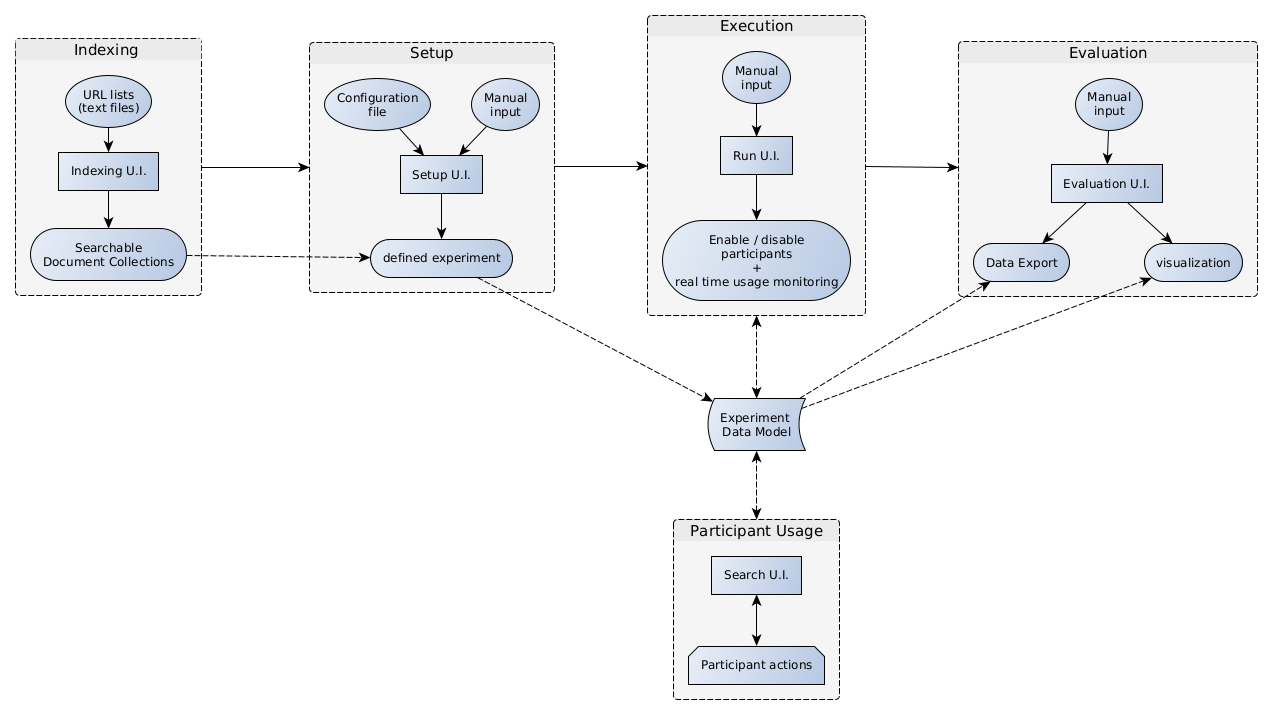
\includegraphics[width=0.7\textwidth]{figures/usage}
\caption{Typical usage workflow}
\label{fig:usage}
\end{figure}


%%%%%%%%%%%%%%%%%%%%%%%%%
\subsection{\textbf{Defining the Document Corpora}} \label{sec:designDefineDocs}
%%%%%%%%%%%%%%%%%%%%%%%%%

In order to define the document collections (corpora) to be used during subsequent experiments, 
an experimenter can upload text files containing lists of web URLs. The files are  stored, so they can be reused 
for defining multiple document collections. Via a popup menu, a new  document collection can be defined by providing a name, 
the collection's language, and the related URL list.
Clicking on the ``index'' button initiates the indexing process, which includes data download and the creation of an index
data structure for retrieval. The details of the indexing process are explained in section \TODO{link actual section}.
\textbf{Figure \ref{fig:indexing}} shows the relevant parts of the interface.

\begin{figure}[h]
     
     \centering
     \begin{subfigure}[b]{0.6\textwidth}
         \centering
         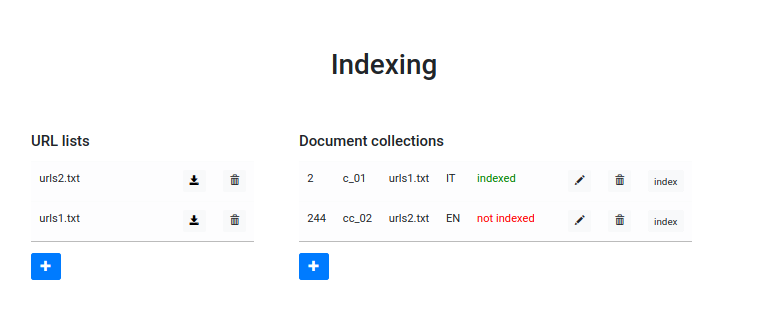
\includegraphics[width=.8\linewidth]{figures/indexing1}
         \caption{indexing  u.i}
         \label{fig:indexingA}
     \end{subfigure}
     \begin{subfigure}[b]{0.3\textwidth}
         \centering
         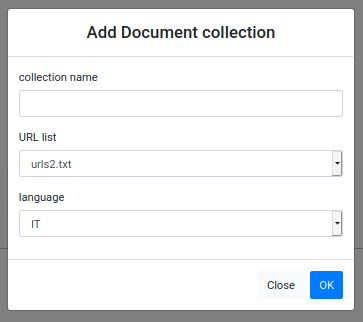
\includegraphics[width=.6\linewidth]{figures/indexing2}
         \caption{popup for defining  document collections}
         \label{fig:indexingB}
     \end{subfigure}
     \caption{Indexing UI page}
     \label{fig:indexing}

\end{figure}


%%%%%%%%%%%%%%%%%%%%%%%%%
\subsection{\textbf{Setting up an Experiment}} \label{sec:designExpSetup}
%%%%%%%%%%%%%%%%%%%%%%%%%

The UI for experiment setup allows defining the details of an experiment to be carried out. This step involves creating
test groups with associated participants and document collections. Groups can be defined either manually or by using 
an uploaded configuration file. In both cases, the test group configuration can later be edited manually. 
The interface allows linking each group to a set of previously indexed document collections. Optionally a document collection
can be set for each test group as predefined result list to be returned after the the first query.
If the experiment is to be executed in the context of a \emph{Qualtrics} survey, the participants don't need to be specified, as they are
defined while they take part in the survey. 
\textbf{Figure \ref{fig:setup}} shows this UI.

\begin{figure}[h!]
\centering
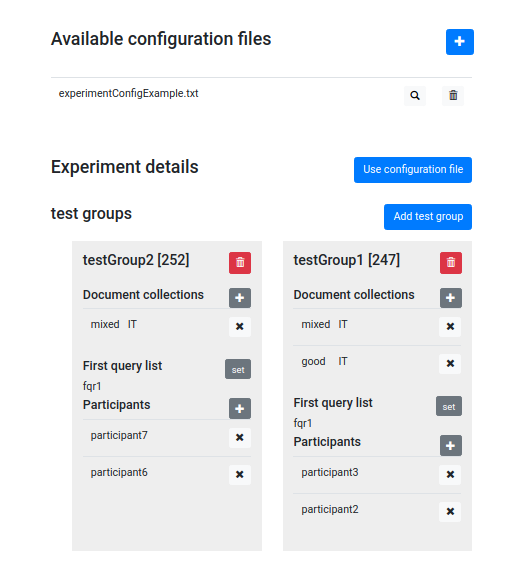
\includegraphics[width=0.6\textwidth]{figures/setup}
\caption{U.I. for experiment setup}
\label{fig:setup}
\end{figure}


%%%%%%%%%%%%%%%%%%%%%%%%%
\subsection{\textbf{Running an Experiment}} \label{sec:designExpRun}
%%%%%%%%%%%%%%%%%%%%%%%%%

The UI for experiment execution includes a start/stop/reset button, a timer, and a tabular display 
showing the current participant activities. Clicking the start button starts the timer, enables the participants to log in, and
initiates the data collection process. While the experiment is running, all queries and click carried out by the
participants are stored as database records including a timestamp, user id, group id, and query/document related data.
The details of the data collection mechanism are described in section \ref{sec:data}.
When the stop button is clicked the participants are logged out and all transient data is saved to the database.
After the experiment is complete the related evaluation page becomes available.
In case something goes wrong, the experiment can be reset. This causes all collected data to be deleted, while the
experiment's configuration is preserved.
\textbf{Figure \ref{fig:run}} shows the user interface.

\begin{figure} [h]
\centering
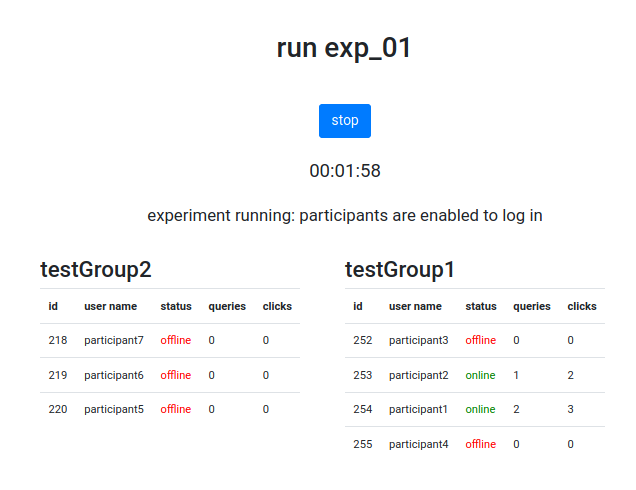
\includegraphics[width=0.6\textwidth]{figures/run}
\caption{UI for experiment execution}
\label{fig:run}
\end{figure}

%%%%%%%%%%%%%%%%%%%%%%%%%
\subsection{\textbf{Search Interface Available to Participants}} \label{sec:designSearchUi}
%%%%%%%%%%%%%%%%%%%%%%%%%

The interface available to the participants looks similar to the main page of most known search engines. It simply
includes a search text bar and a button for entering queries and displays the results as a list of
links accompanied by short summaries (snippets) with highlighted query terms. 
\textbf{Figure \ref{fig:searchUi}} shows the UI after a query has been entered.

\begin{figure} [h]
\centering
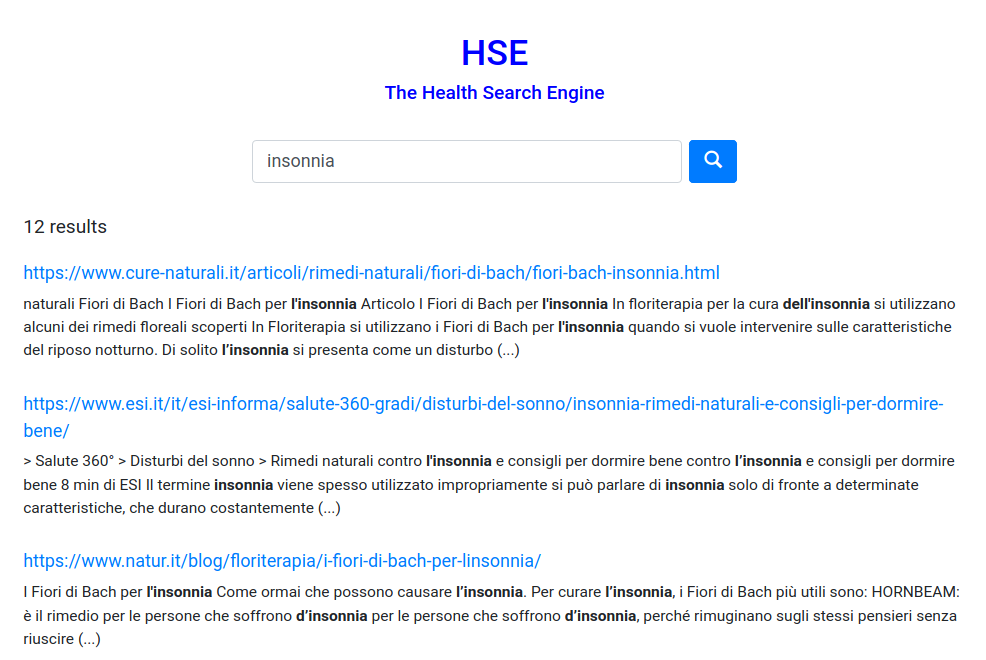
\includegraphics[width=0.7\textwidth]{figures/searchUi}
\caption{User interface available to participants}
\label{fig:searchUi}
\end{figure}

%%%%%%%%%%%%%%%%%%%%%%%%%
\subsection{\textbf{Experiment Evaluation}} \label{sec:designExpEval}
%%%%%%%%%%%%%%%%%%%%%%%%%

After an experiment has been conducted, the  related evaluation interface becomes available. From this page,
experimenters can inspect the experiment's results and export  the complete raw data
or preprocessed data summaries.

The raw data can be exported either in \emph{CSV} or \emph{JSON} format and consists of a list of all user actions that occurred during the experiment. 
Each record has a timestamp, a user id, and a group id. Query event records include the query text and the proportions in which
the data collections are represented  in the result list. Document click event records include the document id, its URL, and
the collection to which the given document belongs.

The data summaries include overall experiment statistics and per-group statistics. Moreover, the individual user histories can be 
exported in the same formats as the raw data.
Per-experiment statistics include the total count of clicks and queries as well as averages, medians, and standard deviations
for queries per user, clicks per user, clicks per query, time per query, and time per click.
Per group statistics include the same metrics as the per-experiment statistics, plus totals, averages, medians, and standard deviations
for clicks per document collection. Details on the raw data format and the computed statistics are described in \ref{sec:data}.

%%%%%%%%%%%%%%%%%%%%%%%%%%%%%%%%%%%%%%%%%%%%%%%%%%
\section{\textbf{Raw Data Generation and Computed Statistics}} \label{sec:data}
%%%%%%%%%%%%%%%%%%%%%%%%%%%%%%%%%%%%%%%%%%%%%%%%%%

%%%%%%%%%%%%%%%%%%%%%%%%%
\subsection{\textbf{Raw Data Records}} \label{sec:dataRaw}
%%%%%%%%%%%%%%%%%%%%%%%%%

The usage tracking system is based on generating records whenever a participant performs a relevant action. The application
distinguishes three kinds of usage events: session events (log in / log out), query events (generated when a participant
submits a search query), and document click events (generated when a participant visits a page by clicking on an item in the search results list). All usage events include the following data fields:

    \begin{itemize}

        \item
        A unique id.

        \item
        A timestamp indicating the precise time when the event occurred.

        \item
        The id of the participant who triggered the event.

        \item
        The id and name of the test group which the participant belongs to.

        \item
        The event type (one of ``SESSION'', ``QUERY'', or ``DOC\_CLICK'').


    \end{itemize}

Query events contain the following additional fields:

    \begin{itemize}

        \item
        The query string entered by the participant.

        \item
        The total number of results retrieved.

        \item
        The number of results retrieved from each of the available document collections.

    \end{itemize}

Document click events contain the following additional fields:

    \begin{itemize}

        \item
        The URL of the corresponding web page.

        \item
        The document's id assigned during indexing.

        \item
        The id and name of the document collection the given document belongs to.

        \item
        The document's rank (i.e. its position within the search results list).


    \end{itemize}

The raw data records can be exported via the experiment's evaluation page in \emph{CSV} or
\emph{JSON} format in order to be used for statistical analysis. Some basic metrics are
computed by the application, as described in the following subsection, and displayed on the
evaluation page.

%%%%%%%%%%%%%%%%%%%%%%%%%
\subsection{\textbf{Computed data}} \label{sec:dataPerExperiment}
%%%%%%%%%%%%%%%%%%%%%%%%%

For each experiment the following quantities are considered:

    \begin{itemize}

        \item
        The total number of query events occurred.

        \item
        The total number of document click events occurred.

        \item
        Mean, median and standard deviation of the number of queries per user.

        \item
        Mean, median and standard deviation of the number of document clicks per user.

        \item
        Mean, median and standard deviation of the number of clicks per query.

        \item
        Mean, median and standard deviation of the time spent per document \\ (duration between a document click event and the next usage event performed by the same participant)

        \item
        Mean, median and standard deviation of the time spent per query \\ (duration between a query and the next query or logout).

    \end{itemize}

The same metrics are available for each test group, allowing for interesting comparisons. Moreover, for each test group, the distribution
of documents visited and time spent over the document collections from which the results are drawn is represented.
Section \ref{impl:dataSummaries} describes the details of how these measures are computed.

\newpage

%%%%%%%%%%%%%%%%%%%%%%%%%%%%%%%%%%%%%%%%%%%%%%%%%%
\section{\textbf{Software Architecture and Employed Frameworks}} \label{sec:arch}
%%%%%%%%%%%%%%%%%%%%%%%%%%%%%%%%%%%%%%%%%%%%%%%%%%

The project requirements implied building a web application including a text information retrieval system. Both aspects are highly complex and it would not be reasonable to build such an application completely from scratch, so I
needed to rely on appropriate libraries and frameworks. As a general framework I chose \emph{SpringBoot} 
(a \emph{Java} framework for web applications) \cite{springBootHome}, since
I had used it in past projects and knew that it includes very useful features for handling the main issues related to
serving web pages, interacting with a database, and providing endpoints for \emph{Ajax} calls and \emph{WebSocket} services.
For the information retrieval part, I chose \emph{Apache Lucene} \cite{luceneHome} in conjuction with the \emph{Tika} content analysis toolkit \cite{tikaHome}
(used for text extraction). \emph{Lucene} includes all functionalities needed for indexing and retrieval,
and since it is a \emph{Java} library, it can be easily integrated into a \emph{SpringBoot} application. As a database management system
I chose \emph{MySql} \cite{MySQLhome}.
For managing the dependencies and configuring the build process of the SpringBoot application I used the \emph{Apache Maven}
project management tool, which allows a simple configuration based on a single file (\emph{pom.xml}).
For an easy and portable deployment I configured \emph{Maven} to create a \emph{Docker} \cite{dockerHome} image when the application is built;
this makes the configuration and system requirements on the on the production server as simple as possible.  
For the client-side I used the \emph{jQuery}\cite{jQueryHome} library in order to keep the \emph{JavaScript} code simple
and having an easy way to perform \emph{AJAX} (Asynchronous JavaScript and XML) calls. I also employed the
\emph{Bootstrap} \cite{bootstrapHome} toolkit for the graphical aspects of the front-end interfaces.
The next two subsections explain how the different parts of the system interact.

%%%%%%%%%%%%%%%%%%%%%%%%%
\subsection{\textbf{Overall Architecture}} \label{sec:archOverall}
%%%%%%%%%%%%%%%%%%%%%%%%%

The core of the system is the \emph{SpringBoot} application, whose tasks include serving web content
(HTML, CSS and JS files) upon HTTP requests, managing users and authentication (users with different roles have access to different interfaces),
updating database records upon form submissions and \emph{AJAX} calls, managing \emph{WebSocket} services, and
providing interfaces for uploading and downloading files. \textbf{Figure \ref{fig:archGeneral}} summarizes the
overall system architecture; the following sections explain why various interactions are required and how they are implemented using the
chosen frameworks and libraries.

\begin{figure}[h!]
\centering
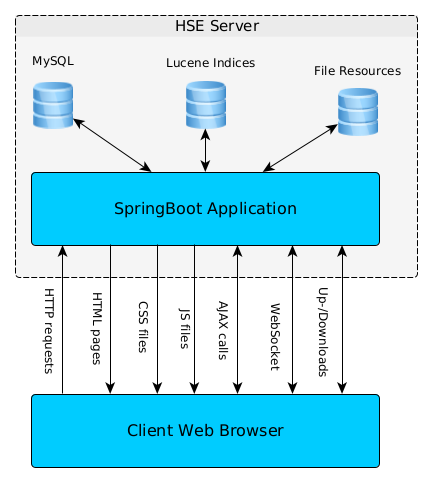
\includegraphics[width=0.6\textwidth]{figures/archGeneral}
\caption{General System Architecture}
\label{fig:archGeneral}
\end{figure}

\subsubsection{\textbf{Serving Web Content}}

For serving web content, the framework leverages the \emph{Thymeleaf} \cite{thymeleafHome} template engine and uses so called \emph{Controller}
classes for reacting to \emph{HTTP} requests. Within a controller class, methods with
the annotation \emph{@RequestMapping}, are defined for responding to requests for specific \emph{URL} paths.
These methods can return either an object of the class \emph{ModelAndView}, allowing to inject
variables into the templates, or simply a string representing the name of a template file. 

\emph{Thymeleaf} template files consist mainly of \emph{HTML}, but allow also syntax for useful operations to
be performed server-side, such as including variables (which can be complex \emph{Java} objects),
selectively include \emph{HTML} elements depending on conditions, include multiple \emph{HTML} elements
by iterating over a list, or defining reusable elements (fragments), which can be imported in
multiple other template files. \emph{JavaScript}, \emph{CSS}, and other static files can be included
using classical \emph{HTML} syntax. The template engine automatically finds and loads the templates as well as
static files, as long as they are placed in the project's \emph{resources} directory.

\subsubsection{\textbf{REST Endpoints for \emph{Ajax} requests}}

In several parts of the application, the front-end code needs to send information to the
server (e.g. when defining experiments and test groups), or retrieve
information from the server (e.g. the current state of an experiment). This is done via
\emph{Asynchronous JavaScript and XML} (\emph{Ajax}).
The main advantage of \emph{Ajax} is that it allows interactions between server and client that are independently from
displaying a web page \cite{ajaxWikipedia}. This makes the application much more efficient, because the alternative would be reloading
the same page whenever some data must be sent or retrieved.
There are several possible implementations for \emph{Ajax}, but the one most frequently used nowadays is based on
\emph{XMLHttpRequest} and transfers data in \emph{JavaScript Object Notation} (\emph{JSON}).

Systems that use \emph{Ajax} for transferring data and consider the semantics of the \emph{HHTP} request's method
(GET, POST, PUT, DELETE and others) are often referred to as \emph{REST API} or \emph{RESTful} service,
where \emph{REST} stands for ``Representational State Transfer'' \cite{restWikipedia}. Implementing the
server-side of such a system can be done quite easily in \emph{SpringBoot}, since it includes a mechanism
designed specially for this purpose: the \emph{Jackson ObjectMapper} converts \emph{Java objects} to \emph{JSON} strings
and vice versa, so when writing a \emph{Controller} class, all data is represented in \emph{Java}, while
the front-end sends and receives \emph{JSON} \cite{baeldungJackson}. 

\subsubsection{\textbf{WebSocket for interactive communication}}

Though \emph{Ajax} works perfectly for pulling information from the server to the client or pushing it from the 
client to the server, the actions can only be triggered on the client-side. But in my application there
are a few situations in which it must work the other way around. One such case is updating the participant actions displayed to
experimenters on the experiment's run page during execution: when a user performs a query or clicks on a link 
the corresponding event is stored on the server, and the experimenter's page must be somehow notified that an event occurred.

The classical way to solve this issue (before the \emph{WebSocket} protocol existed) was to poll for the
current state. In my case this would have meant performing an \emph{Ajax} call at regular and possibly short intervals 
(e.g. once a second) in order to retrieve the current state of the experiment (including the participant's action counts)
and update the displayed data.
This approach works, but is quite inefficient, since information is transferred and computations are done even if nothing
has changed.

The \emph{WebSocket} protocol offers an elegant alternative \cite{websocketWikipedia}: it provides full-duplex communication channels
over a single \emph{TCP} connection by using a modification of the \emph{HTTP} protocol. Including the \emph{WebSocket} functionality
in a web application is quite simple. In \emph{SpringBoot} it requires adding the dependency for \emph{spring-boot-starter-websocket},
creating a class which implements the \emph{WebSocketMessageBrokerConfigurer} interface in order to configure the channels, and
send messages by using the \emph{@SendTo} annotation or an instantiation of \emph{SimpMessagingTemplate}.
On the front-end, the \emph{SockJs} library provides functions for connecting and subscribing to specific channels, and it is 
straight-forward to execute any \emph{JavaScript} code whenever a message is received.  


\subsubsection{\textbf{File Upload and Download}}

In several situation my application must enable uploading files and storing them on the server or downloading files 
generated on the server to the client system: experimenters need to upload \emph{URL} lists for creating document collections as well as 
configuration files for defining test groups, and they must be able to download the data collected during an experiment.

File upload can be done in \emph{Spring} by setting parameter of type \emph{MultipartFile}. This object has a method
\emph{getInputStream()}, which returns a standard \emph{Java} stream that can be written to the file system e.g. using
the \emph{java.nio.file.Files} API. File download is equally simple: the \emph{Java InputStream} from a file can be copied to
the \emph{OutputStream} associated with a \emph{HttpServletResponse} object (passed as parameter to a \emph{Controller} method)
e.g. using \emph{FileCopyUtils} \cite{springFileUpload}. On the front-end one can upload files via a form including a
\emph{HTML} input tag with \texttt{type="file"}. Files can be downloaded using a link.

\subsubsection{\textbf{Database interactions with \emph{Spring Data JPA}}}

The application heavily relies on data storing and retrieving structured data: user data
needs to be stored for enabling access control, metadata about document collections and experiment settings
must be stored both for regulating the experiment's execution process, and during execution the participant's
actions must be logged. The best way for implementing this kind of functionality is by using a
\emph{Database Management System (DBMS)} which allows for efficient storage and retrieval.
I chose \emph{MySql} for this purpose because I already had some experience with it, and there is plenty of documentation online on how to 
interact with it from a \emph{SpringBoot} application \cite{springJpaReference} \cite{springJpaTutorial}.

In fact \emph{SpringBoot}'s \emph{Data JPA} features allow to define entities as \emph{Java} classes without ever using the \emph{DBMS} directly.
The library automatically generates the corresponding tables: classes are mapped to tables, and data members are mapped to fields. Also advanced functionalities such as one-to-many or many-to-many realationships
can be defined in pure \emph{Java}; even inheritance structures are mapped automatically from \emph{Java} to the \emph{DBMS}. The
details can be configured using annotations.
Data access is managed via repositories which are defined as \emph{Java} interfaces.

\subsubsection{\textbf{Integrating \emph{Lucene} indexing and retrieval}}

The \emph{Lucene} library can be easily added to the project by specifying it as a dependency in the \emph{Maven} configuration.
Once the library is available, its classes can be instantiated and methods can be called. Both indexing and retrieval can
be implemented based on classical \emph{Java} data structures. Details on how
I used the library for the specific needs of my application are described in sections \ref{sec:implIndexing} 
and \ref{sec:implRetrieval}.

%%%%%%%%%%%%%%%%%%%%%%%%%
\subsection{\textbf{Internal Architecture of the \emph{SpringBoot} Application}} \label{sec:archBackend}
%%%%%%%%%%%%%%%%%%%%%%%%%

\emph{SpringBoot} does not enforce a particular architecture or package structure, but a pattern which I often encountered is a combination
of a layered structure in which each layer communicates only with the layer directly below, and a package-per-feature structure, where
tightly coupled classes are placed in the same package. My application roughly follows this approach, using the following layers:

    \begin{description}

        \item[Web Layer]
        Top layer of the hierarchy, containing \emph{Controller} classes with methods to handle web requests and API calls.
        This layer contains a single package named ``endpoints''. This layer uses the functionalities provided by the service layer.

        \item[Service Layer]
        This layer provides abstractions for lower level functionalities such as file access, database interactions user management and
        implementations of custom features like indexing, retrieval, and experiment configuration / evaluation.
        Also this layer consists of a single package named ``services'', containing classes for accessing the specific functionalities
        provided by the data access and processing layer below.

        \item[Data / Processing Layer]
        This layer contains the actual implementation of the features exposed by the service layer, and is divided into packages 
        grouping related functionalities. The following packages belong to the implementation layer:
        ``db'' with sub-packages ``entities'' and ``repositories'' (providing access to the \emph{DBMS}), 
        ``storage'' (containing classes for reading and writing files in several formats),  
        ``indexing'' and ``retrieval'' (for using the features of the \emph{Lucene} library).

    \end{description}

Functionalities which are used application-wide are to be considered outside the layered structure. These include
custom exceptions and an exception-handling mechanism (grouped in a package named ``exceptions''), as well as global
configuration classes (grouped in a package named ``config''). \textbf{Figure \ref{fig:archLayers}} shows the
layered architecture of the application: green rectangles represent packages, blue ovals represent classes,
solid lines represent connections through instantiation or method calls, dashed lines indicate other interactions.
In the following subsections I describe each layer in more detail.


\begin{figure}[h!]
\centering
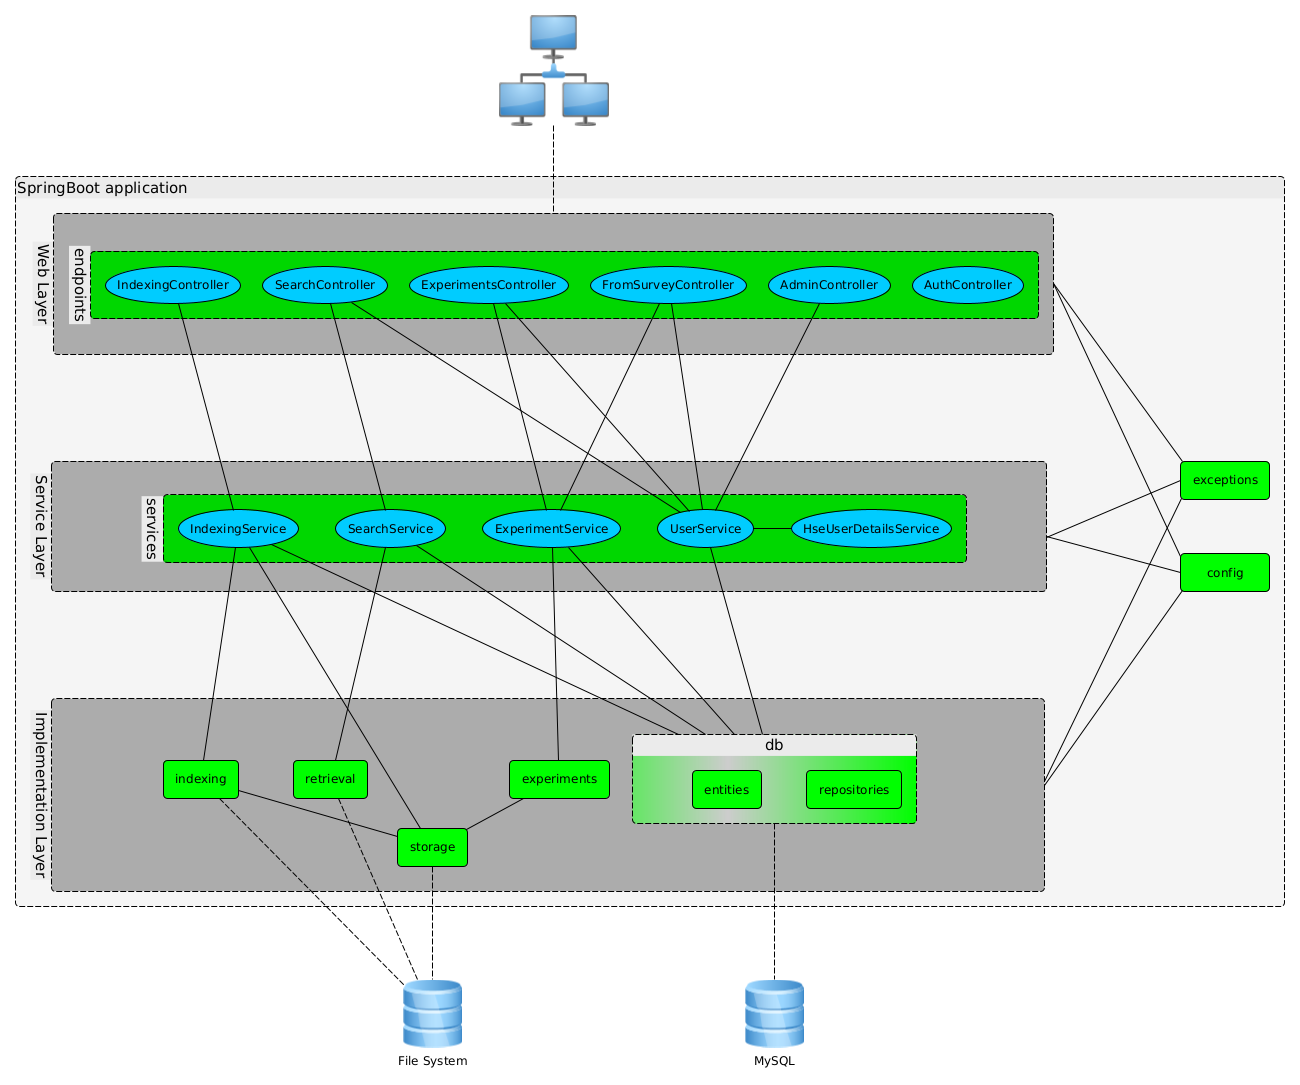
\includegraphics[width=0.9\textwidth]{figures/archLayers}
\caption{Layered architecture of the back-end application}
\label{fig:archLayers}
\end{figure}

%%%%%%%%%%%%%%%%%%%%%%%%%
\subsection{\textbf{The Web Layer: Controller Classes for Handling \emph{HTTP} requests}} \label{sec:archWebLayer}
%%%%%%%%%%%%%%%%%%%%%%%%%

The \emph{Web Layer} contains the single package \texttt{endpoints}; functionalities are split into classes depending on the
user interface from which they are supposed to be called and the services they depend on.
The \texttt{endpoints} package contains the following classes:
\texttt{AdminController},
\texttt{AuthController},
\texttt{ExperimentsController},
\texttt{FromSurveyController}, \\
\texttt{IndexingController}, and
\texttt{SearchController}.

\subsubsection{\textbf{AdminController}}

The class \texttt{AdminController} handles requests to \emph{URL}s with prefix ``\texttt{/admin}'' available to users with \texttt{Administrator} role.
The functionalities of this controller include serving the \texttt{admin} \emph{UI} page and reacting to \emph{Ajax} requests coming from it.
The purpose of this interface is creating, updating or removing administrators, experimenters, 
and participants by using methods of the \texttt{UserService} class
from the service layer. For details on users and their roles see section \ref{sec:implUsers}.

The class contains the following public methods:

    \begin{description}

        \item[\texttt{getAdminUi}]
        (annotated with \texttt{@GetMapping("/ui")}) 

        serves the \texttt{admin} \emph{UI} page. It takes no explicit parameters and returns an object
        of class \texttt{ModelAndView}. The lists of all users, separated by role, are added to the returned object as template variables.

        \item[\texttt{postAdministrator}]
        (annotated with \texttt{@PostMapping("/administrators")}) 

        takes a parameter of type \texttt{Administrator},
        which is passed as request body in an \emph{Ajax} \emph{POST} request. It adds
        the corresponding new administrator to the database by calling the \texttt{UserService} and returns a \texttt{ResponseEntity}
        containing the newly created user. 

        \item[\emph{POST} mappings for \texttt{Experimenter} and \texttt{Participant}] analogous to the \texttt{postAdministrator} method
        described above, but for handling users with \texttt{Experimenter} or \texttt{Participant} role.

        \item[\texttt{putAdministrator}] 
        (annotated with \texttt{@PutMapping("/administrators")}) takes a parameter of type \texttt{Administrator},
        which is passed as request body in an \emph{Ajax} \emph{PUT} request. It updates the corresponding
        user in the database (e.g. changing the user name or password) and returns the updated object wrapped
        in a \texttt{ResponseEntity}.

        \item[\emph{PUT} mappings for \texttt{Experimenter} and \texttt{Participant}] analogous to  the \texttt{putAdministrator} method
        described above, but for handling users with \texttt{Experimenter} or \texttt{Participant} role.

        \item[\texttt{deleteAdministrator}]
        (annotated with \texttt{@DeleteMapping("/administrators")}) 

        takes a parameter of type \texttt{Administrator},
        which is passed as request body in an \emph{Ajax} \emph{DELETE} request. The corresponding user is
        deleted from the database. The method returns a \texttt{ResponseEntity} containing the deleted user.

        \item[\emph{DELETE} mappings for \texttt{Experimenter} and \texttt{Participant}] analogous to  the \texttt{deleteAdministrator} method
        described above, but for handling users with \texttt{Experimenter} or \texttt{Participant} role.

        \item[delteAllExperimenters] 
        (annotated with \texttt{@DeleteMapping("/experimenters/all")}) 

        takes no explicit parameters and removes all
        users with \texttt{Experimenter} role from the database. The method returns a \texttt{ResponseEntity} containing a string
        to confirm that the operation has succeeded.

        \item[delteAllParticipants]
        Same as the method described above, but for deleting all users with \texttt{Participant} role.

    \end{description}

\subsubsection{\textbf{AuthController}}

This is a minimal controller class containing a single method for serving the login page. \\ The method returns
an object of class \texttt{ModelAndView}.

\subsubsection{\textbf{SearchController}}

The \texttt{SearchController} is in charge of serving the main search engine \emph{UI} available to
participants, and redirecting them to a specific search result when they click on a link or to a logout
page if the experiment is terminated. These actions are performed by calling the \texttt{SearchService} and
\texttt{UserService} from the service layer through the following methods:

    \begin{description}

        \item[\texttt{getSearchUi}]
        (annotated with \texttt{@GetMapping("/")}) 

        This method serves the main search engine \emph{UI}, optionally including the results of the last query submitted.
        It takes two parameters: an object of class \texttt{org.springframework.security.core.userdetails.User} which
        is generated by the framework and is needed for identifying the calling participant, and optionally
        a \texttt{String} representing the query entered in the search form. 

        If the query string is empty and no query has been submitted before by the given user, the search \emph{UI} with
        empty results list is returned; if a query was submitted before, the last results list is added to the \texttt{ModelAndView}.
        If the query string is not empty, the method checks whether it is the first query (in which case if a predefined first-query
        result list for exists it is used, otherwise the query is processed by the retrieval system and the returned 
        result list is added to the \texttt{ModelAndView}). If the query
        is not the first one and has different content from the first one, the query is processed and the result list is 
        added to the \texttt{ModelAndView}.

        These operations are performed by calling the methods \texttt{handleFirstQuery}, \texttt{handleRepeatedQuery}, 
        and \\ \texttt{handleNewQuery} from the \texttt{SearchService} (see section \ref{sec:archServiceSearch}).

        \item[\texttt{getResultDoc}]
        (annotated with \texttt{@GetMapping("/doc")})
        
        This method serves the result page that is displayed upon clicking on a link in the results list.
        It take the following two parameters: the \emph{URL} of the original web document and its file type
        (\emph{PDF} documents are displayed using a slightly different mechanism than the one used for \emph{HTML}
        documents). These parameters are added to the returned \texttt{ModelAndView}.

        \item[\texttt{postBrowseEvent}]
        (annotated with \texttt{@GetMapping("/doc")})

        This method is to be called via an \emph{Ajax POST} request in order to generate and store a document
        click event. It takes the \texttt{SearchResult} object (see section \ref{sec:implRetrieval}) corresponding to the clicked link 
        and the \texttt{User} object corresponding to the participant as parameters.

    \end{description}

\subsubsection{\textbf{IndexingController}}

The class \texttt{IndexingController} implements all interactions needed for managing \emph{URL} lists
and document collections. It serves the indexing \emph{UI} page and provides endpoints for handling file upload / download
and \emph{Ajax} requests related to the creation, modification, and deletion of document collections by responding
to \emph{HTTP} requests with \emph{URL} prefix \texttt{/indexing}.
It uses the \texttt{IndexingService} from the service layer and contains the following public methods:

    \begin{description}

        \item[\texttt{getIndexingUi}]
        (annotated with \texttt{@GetMapping("/ui")})

        serves the indexing \emph{UI} page. The file names of all saved \texttt{URL} lists and the 
        objects corresponding to all stored document collections are added to the returned \texttt{ModelAndView}.

        \item[\texttt{postUrlList}]
        (annotated with \texttt{@PostMapping("/urlLists")})

        takes an object of type \texttt{MultipartFile} representing a text file as parameter. The file is stored
        by calling the \texttt{addUrlList} method of the \texttt{IndexingService}.

        \item[\texttt{deleteUrlList}]
        (annotated with \texttt{@DeleteMapping("/urlLists")})

        takes the name of the \emph{URL} list to be deleted representing a as parameter and deletes the corresponding file
        by calling the \texttt{removeUrlList} method of the \texttt{IndexingService}.

        \item[\texttt{downloadUrlList}]
        (annotated with \texttt{@GetMapping("/urlLists/dl")})

        takes the \texttt{HttpServletResponse} (provided by the framework) and the name of a \emph{URL} list as parameters 
        and makes the corresponding file available for download.
        It does so by getting the file as \emph{Java} \texttt{InputStream} from the \texttt{IndexingService} and
        copying it to the response's \texttt{OutputStream}. 
        
        \item[\texttt{postDocCollection}]
        (annotated with \texttt{@PostMapping("/docCollections")})

        responds to an \emph{Ajax} request containing a \texttt{DocCollection} object as request body.
        It takes the object as parameter, persists it in the database using the \texttt{IndexingService}'s addDocCollection method,
        and returns the saved object wrapped in a \texttt{ResponseEntity}.

        \item[\texttt{updateDocCollection}]
        (annotated with \texttt{@PutMapping("/docCollections")})

        responds to an \emph{Ajax} request containing a \texttt{DocCollection} object as request body.
        It takes the object as parameter, updates it's persistent version in the database using the \texttt{IndexingService}'s 
        updateDocCollection method,
        and updated the saved object wrapped in a \texttt{ResponseEntity}.

        \item[\texttt{deleteDocCollection}]
        (annotated with \texttt{@DeleteMapping("/docCollections")})

        responds to an \emph{Ajax} request containing a \texttt{DocCollection} object as request body.
        It takes the object as parameter, deletes it from the database using the \texttt{IndexingService}'s 
        removeDocCollection method,
        and updated the deleted object wrapped in a \texttt{ResponseEntity}.

        \item[\texttt{buildIndex}]
        (annotated with \texttt{@PostMapping("/buildIndex")})

        responds to an \emph{Ajax} request containing a \texttt{DocCollection} object as request body.
        The indexing process for the given collection is initiated (see section \ref{sec:implIndexing}),
        and an object of type \texttt{IndexingResult}, which summarizes the operations results,
        is returned wrapped in a \texttt{ResponseEntity}. The process is performed by
        calling the \texttt{buildIndex} method from the \texttt{IndexingService}.


    \end{description}


\subsubsection{\textbf{ExperimentsController}}

The class \texttt{ExperimentsController} handles requests to \emph{URL}s with prefix 
``\texttt{/experiments}'' available to users with \\ \texttt{Administrator}
or \texttt{Experimenter} role. Its purposes are serving the \emph{UI} pages for creating, configuring, running, and evaluating
experiments, and handling the related \emph{Ajax} requests. For performing these operation, the class uses the functionalities
provided by the \texttt{ExperimentService} and \texttt{UserService} from the service layer. 

    \begin{description}

        \item[Serving The \emph{UI} Pages]
        The pages for managing experiments are served via the methods \texttt{getExperimentsUi()}, 
        \\ \texttt{getExperimentsSetupUi()},
        \texttt{getExperimentsUi()}, \texttt{getExperimentsRunUi()}, and \texttt{getExperimentsEvalUi()}.
        The first method takes no explicit parameters, while the others require the experiment's id to be passed as a \texttt{URL}
        parameter in the \texttt{HTTP} request because the corresponding pages relate to a single experiment at a time.
        All four methods return an object of class \texttt{ModelAndView}.

        \item[REST API for creating, updating and deleting experiments]
        Experiments can be created, updated and deleted via \emph{AJAX} calls using the \texttt{HTTP} methods
        \emph{POST}, \emph{PUT}, and \emph{DELETE} and providing the experiment object as request body. For
        details on the structure of \texttt{Experiment} objects see section \ref{sec:implExperiments}.

        The methods responsible for these actions are \texttt{postExperiment}, \texttt{putExperiment}, and
        \texttt{deleteExperiment}, each taking a parameter of type \texttt{Experiment} and returning an
        object of the same type wrapped in a \texttt{ResponseEntity}.

    \end{description}

\subsubsection{\textbf{FromSurveyController}}

This controller handles the interaction required for integrating the application into a \emph{Qualtrics} survey;
it responds to \emph{HTTP} requests with \emph{URL} prefix ``/from\_survey''.
It provides a method for serving the search \emph{UI} while automatically logging in a participant, as well as
a \emph{REST API} which allows for creating participants and checking if a given experiment is running. These
operations are performed by calling the \texttt{UserService} and \texttt{ExperimentService} from
the service layer.
Below is a brief description of each method:

    \begin{description}

        \item[getSearchUiFromSurvey]
        (annotated with \texttt{@GetMapping("/")})

        Serves the search \emph{UI} page for participants from a \emph{Qualtrics} survey.
        takes a user id and the survey \emph{URL} as parameters. The id is needed for logging in the corresponding participant
        and load the experiment data,
        while the \emph{URL} is stored for later redirecting the participant back to the survey.

        the method performs the following actions:

        \begin{itemize}

            \item
            The user data corresponding to the given id is retrieved from the database via the \texttt{UserService}.

            \item
            The experiment is loaded using the experiment id stored in the user data.

            \item
            If the given experiment is not running, the user is redirected to an error page by returning the
            corresponding \texttt{ModelAndView} object. 

            This is a fallback for a situation that should not occur,
            since the survey is supposed to check whether the experiment is running before redirecting the user to the application
            (see \textbf{appendix \ref{sec:usageSurvey}}).

            \item
            The participant is logged in and the experiment is updated. If these operations succeed, 
            a \emph{WebSocket} message is sent for updating the experiment's run \emph{UI} and the user is redirected to the search \emph{UI}
            page by returning the corresponding \texttt{ModelAndView} object. Otherwise an exception is returned in the \emph{HTTP} response.
            

        \end{itemize} 

    \end{description}


%%%%%%%%%%%%%%%%%%%%%%%%%
\subsection{\textbf{The Service Layer: Service Classes Providing the Core Functionalities}} \label{sec:archServiceLayer}
%%%%%%%%%%%%%%%%%%%%%%%%%

\subsubsection{UserService}

\subsubsection{IndexingService}

\subsubsection{SearchService}\label{sec:archServiceSearch}

\subsubsection{ExperimentService}

\subsubsection{HseUserDetailsService}


%%%%%%%%%%%%%%%%%%%%%%%%%
\subsection{\textbf{The Data / Processing Layer: Implementation of the Core Functionalities}} \label{sec:archDataLayer}
%%%%%%%%%%%%%%%%%%%%%%%%%



%%%%%%%%%%%%%%%%%%%%%%%%%%%%%%%%%%%%%%%%%%%%%%%%%%
\section{\textbf{Implementation details}} \label{sec:impl}
%%%%%%%%%%%%%%%%%%%%%%%%%%%%%%%%%%%%%%%%%%%%%%%%%%

%%%%%%%%%%%%%%%%%%%%%%%%%
\subsection{\textbf{User Management}} \label{sec:implUsers}
%%%%%%%%%%%%%%%%%%%%%%%%%

%%%%%%%%%%%%%%%%%%%%%%%%%
\subsection{\textbf{Experiment Representation}} \label{sec:implExperiments}
%%%%%%%%%%%%%%%%%%%%%%%%%

%%%%%%%%%%%%%%%%%%%%%%%%%
\subsection{\textbf{Indexing}} \label{sec:implIndexing}
%%%%%%%%%%%%%%%%%%%%%%%%%

%%%%%%%%%%%%%%%%%%%%%%%%%
\subsection{\textbf{Retrieval}} \label{sec:implRetrieval}
%%%%%%%%%%%%%%%%%%%%%%%%%

%%%%%%%%%%%%%%%%%%%%%%%%%
\subsection{\textbf{Data Extraction and Summary Generation}} \label{impl:dataSummaries}
%%%%%%%%%%%%%%%%%%%%%%%%%


%%%%%%%%%%%%%%%%%%%%%%%%%%%%%%%%%%%%%%%%%%%%%%%%%%
\section{\textbf{Future Work}} \label{sec:futureWork}
%%%%%%%%%%%%%%%%%%%%%%%%%%%%%%%%%%%%%%%%%%%%%%%%%%


%%%%%%%%%%%%%%%%%%%%%%%%%%%%%%%%%%%%%%%%%%%%%%%%%%
\section{\textbf{Conclusions}} \label{sec:conclusions}
%%%%%%%%%%%%%%%%%%%%%%%%%%%%%%%%%%%%%%%%%%%%%%%%%%


\newpage

\begin{appendices}

        %%%%%%%%%%%%%%%%%%%%%%%%%%%%%%%%%%%%%%%%%%%%%%%%%%%%%%%%%%%%%%%%%%%%%%%%%%%%%%%%%%%%%%
        \section{Configuration, Build, and Deployment (from HSE Setup and Usage Guide)}
        \label{sec:deployment}
        %%%%%%%%%%%%%%%%%%%%%%%%%%%%%%%%%%%%%%%%%%%%%%%%%%%%%%%%%%%%%%%%%%%%%%%%%%%%%%%%%%%%%%

        %%%%%%%%%%%%%%%%%%%%%%%%%%%%%%%%%%%%%%%%%%%
        \subsection{Dependencies}

        The system on which you build the application must have the following software installed:

        \begin{itemize}

        \item Java JDK 11

        \item Apache Maven 3.6.3

        \item Docker version 20.10.1

        \end{itemize}

        If you need to run the application locally without using docker, also \emph{MySql} is required. 

        The server on which the application is to be deployed only needs \emph{Docker} and \emph{Docker Compose}.

        %%%%%%%%%%%%%%%%%%%%%%%%%%%%%%%%%%%%%%%%%%%
        \subsection{Configuration Files}

        \subsubsection{Maven configuration: pom.xml}

        The build settings used by \emph{Maven} are defined in \texttt{/hse/pom.xml}. This file contains some general information
        about the project, such as name and version, as well as a list of java packages and \emph{Maven} plugins that are 
        downloaded and set up at build time. The File also declares two profiles (``dev'' and ``prod''). The ``dev'' profile 
        is intended for creating a local build to be used during development, while the ``prod'' profile is to be used for building the deployment version.
        The profiles are linked to specific configuration files which contain various settings such as server ports and global
        constants: when the profile ``dev'' is selected, the application uses the file 

\texttt{/hse/src/main/resources/application-dev.properties};
        when ``prod'' is selected, \texttt{/hse/src/main/resources/application-prod.properties}. 

        By default the ``dev'' profile is selected;
        for using the ``prod'' profile, the flag \texttt{-Pprod} is to be included in the \emph{Maven} command 
        (e.g. \texttt{mvn -Pprod clean install}).

        \subsubsection{Specific configurations in \texttt{.properties} files}

        The directory \texttt{/hse/src/main/resources/} contains three files with extension \texttt{.properties}:

        \texttt{application.properties}, \texttt{application-dev.properties} and \texttt{application-prod.properties}.
        The first one contains settings that are applied independently of the selected profile, while the other
        two contain profile-specific settings. The crucial settings to be considered at build time are the 
        \texttt{spring.datasource.xxx} properties, which indicates the database which the application is going to connect to, and 
        the \texttt{baseUrl} parameter, which indicates the prefix used at server-level.
        For instance, in the \texttt{application-prod.properties} as I have set it up, the data source is pointing to a \emph{MySql} Docker container,
        and the base URL is set to \texttt{/hse/} since I deploy it on \texttt{http://www.robix-projects.org/hse/}. 
        In the \texttt{application-dev.properties} file the data source points to a local \emph{MySql} instance and the baseUrl is \texttt{/}.

        The other properties indicate directory paths and should not need to be modified.

        \subsubsection{docker-compose.yml}

        The simplest way to run the application on a server is by using \emph{Docker Compose}. The way in which the containers are created from the images
        and the internal ports used are defined in 
        \texttt{/hse/docker-compose.yml}.

        %%%%%%%%%%%%%%%%%%%%%%%%%%%%%%%%%%%%%%%%%%%
        \subsection{Creating a local build}

        \subsubsection{Preparing the database}

        In order to run the application locally, a \emph{MySql} database service running on port 3306 is required. The service must contain a database
        named \texttt{hse\_db} and should be accessible via username \texttt{root} and password \texttt{root}. The tables
        are created automatically at application startup. If you need to use other login credentials, or the service is running on another port, these
        parameters can be set in \texttt{application-dev.properties}.

        \subsubsection{Issuing the build command}

        The command
        \begin{verbatim}
        mvn clean install
        \end{verbatim}
        initiates the build process. The process involves executing several test suites, which should work without failure. In case
        the tests fail (e.g. due to path incompatibilities or missing files) the tests can be skipped using the \texttt{-DskipTests} flag:
        \begin{verbatim}
        mvn -DskipTests clean install
        \end{verbatim}

        \subsubsection{Running the application}

        Once the application is built, it can be run in several ways. During development, it is convenient to run it from the IDE (in
        \emph{Eclipse} package explorer, right-click on project $\rightarrow$ Run As $\rightarrow$ Spring Boot App). Alternatives are to run it from command-line using \emph{Maven}:
        \begin{verbatim}
        cd hse/
        mvn spring-boot:run
        \end{verbatim}
        or using \emph{Java}:

        \begin{verbatim}
        cd hse/target/
        java -jar hse-0.1.jar
        \end{verbatim}

        %%%%%%%%%%%%%%%%%%%%%%%%%%%%%%%%%%%%%%%%%%%
        \subsection{Example deployment on \emph{Ubuntu Server} with \emph{Apache2}}

        \subsubsection{Create and transfer the \emph{Docker} image}

        The first step consists of creating the application's image by issuing

        \begin{verbatim}
        cd hse/
        mvn -Pprod clean install
        \end{verbatim}

        At this point, the output of \texttt{docker image ls} should contain a line similar to:

        \begin{verbatim}
        REPOSITORY           TAG       IMAGE ID       CREATED             SIZE
        robix82/usi.ch-hse   0.1       c2137e7cc110   37 seconds ago      758MB
        \end{verbatim}

        Once the image is created it can be exported as a \texttt{.tar} file by issuing

        \begin{verbatim}
        docker save robix82/usi.ch-hse:0.1 > hse.tar
        \end{verbatim}

        Finally the \texttt{.tar} file and \texttt{/hse/docker-compose.yml} must be copied to the server, e.g. using \texttt{scp}.

        \subsubsection{Load the image and start the application}

        On the server, the image from the \texttt{.tar} file can be loaded with

        \begin{verbatim}
        docker load < hse.tar
        \end{verbatim}

        With the image loaded, the application can be started by issuing

        \begin{verbatim}
        docker-compose up &
        \end{verbatim}

        from the directory containing the \texttt{docker-compose.yml} file. The required \emph{MySql} image will
        be downloaded and initialized automatically.

        At this point, the application is reachable on port 8081 (the port can be configured in \texttt{docker-compose.yml}).

        \subsubsection{Apache2 configuration}

        In order to make the application reachable on the server's external address with a custom prefix, it is necessary to
        configure a virtual host using Apache's \texttt{mod\_proxy} module. For details on \texttt{mod\_proxy}, please
        refer to \\ \href{https://www.digitalocean.com/community/tutorials/how-to-use-apache-http-server-as-reverse-proxy-using-mod_proxy-extension}{https://www.digitalocean.com/community/tutorials/...} \\

        The virtual host configuration is done by placing a file (in this example \texttt{hse.conf}) in \texttt{/etc/apache2/sites-available/} and creating
        a symlink to it in \texttt{/etc/apache2/sites-enabled/}:

        \begin{verbatim}
        ln -s /etc/apache2/sites-available/hse.conf /etc/apache2/sites-enabled/
        \end{verbatim}

        The content of the \texttt{.conf} file should look similar to

        \begin{verbatim}
        <VirtualHost *:80>

          ServerName www.robix-projects.org
          ProxyPreserveHost On

          ProxyPass /hse/ http://127.0.0.1:8081/
          ProxyPassReverse /hse/ http://127.0.0.1:8081/

        </VirtualHost>
        \end{verbatim}

        This configuration makes the application available under \texttt{http://www.robix-projects.org/hse}. Notice that
        the prefix \texttt{/hse/} must match the \texttt{baseUrl} property in \texttt{application-prod.properties}
        and the port (8081 in this example) must correspond to the port defined in \texttt{docker-compose.yml}. 

        %%%%%%%%%%%%%%%%%%%%%%%%%%%%%%%%%%%%%%%%%%%%%%%%%%%%%%%%%%%%%%%%%%%%%%%%%%%%%%%%%%%%%%
        \section{Usage (from HSE Setup and Usage Guide)}
        \label{sec:usage}
        %%%%%%%%%%%%%%%%%%%%%%%%%%%%%%%%%%%%%%%%%%%%%%%%%%%%%%%%%%%%%%%%%%%%%%%%%%%%%%%%%%%%%%


        %%%%%%%%%%%%%%%%%%%%%%%%%%%%%%%%%%%%%%%%%%%
        \subsection{Users, Roles, and their Definition \small{(/admin/ui)}}

        The application distinguishes three types (roles) of users: \emph{Administrators}, \emph{experimenters}, and \emph{participants}.
        Depending on a user's role, different UI elements are visible or accessible: participants can access only the search interface; 
        experimenters have access to the indexing and the experiment setup interfaces; administrators have access to all interfaces,
        including a page for creating, updating, and removing administrators and experimenters. Participants can be defined
        by administrators or experimenters when an experiment is set up, or automatically if the experiment is run within
        a \emph{Qualtrics} survey.

        If the application is newly installed, a default user with \emph{Administrator} role is created. This user can log in using
        the user name ``\emph{admin}'' and password ``\emph{admin}''.

        %%%%%%%%%%%%%%%%%%%%%%%%%%%%%%%%%%%%%%%%%%%
        \subsection{URL lists and Document collections \small{(/indexing/ui)}}

        Before an experiment can be set up, at least one document collection must be available. These can be created on the \emph{indexing}
        UI page available to experimenters and administrators (see \textbf{Figure \ref{fig:indexingUi}}). Creating a document collection involves
        the following steps:
        \begin{itemize}

        \item Upload a URL list, i.e. a text file (.txt) containing one URL per line.

        \item Define a doc collection by setting its name, the URL list to be used, and the language (\emph{IT} or \emph{EN})
                of the web pages.

        \item Start the indexing process. This may take a long time since it involves downloading all the pages over the network;
              while testing I observed times in the order of one second per URL.

        \end{itemize}

        Document collections will later be assigned 
        to test groups, so the search engine returns different results depending on which test group a participant belongs to. Optionally
        a document collection can be set as a fixed result for the first query; in this case, the first query submitted by a
        participant returns this entire document collection, in the order in which the URLs are set in the list used for generating it.

        \begin{figure} [h]
        \centering
        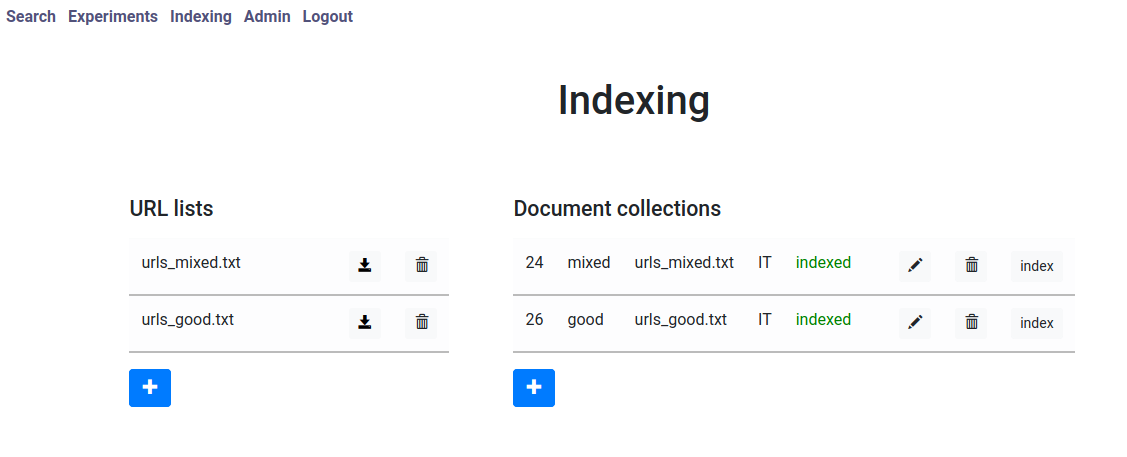
\includegraphics[width=0.9\textwidth]{figures/indexingUi}
        \caption[]{User interface for creating document collections}
        \label{fig:indexingUi}
        \end{figure}

        \newpage


        %%%%%%%%%%%%%%%%%%%%%%%%%%%%%%%%%%%%%%%%%%%
        \subsection{Experiment Definition \small{(/experiments/ui)}}

        The \emph{/experiments/ui} page lists all defined experiments. Each line shows the experiment's unique id (needed for running
        with a \emph{Qualtrics} survey), its title, mode (\emph{stand\_alone} or \emph{Qualtrics}), the assigned experimenter, the date on which it was defined, 
        its status (one of \emph{created}, \emph{ready}, \emph{running}, or \emph{complete}), and buttons leading to the UI for configuration,
        execution, and evaluation. The buttons are enabled or disabled depending on the experiment's status. \textbf{Figure \ref{fig:experimentsUi}}
        shows the experiments interface.

        \begin{figure} [h]
             \centering
             \begin{subfigure}[b]{0.8\textwidth}
                 \centering
                 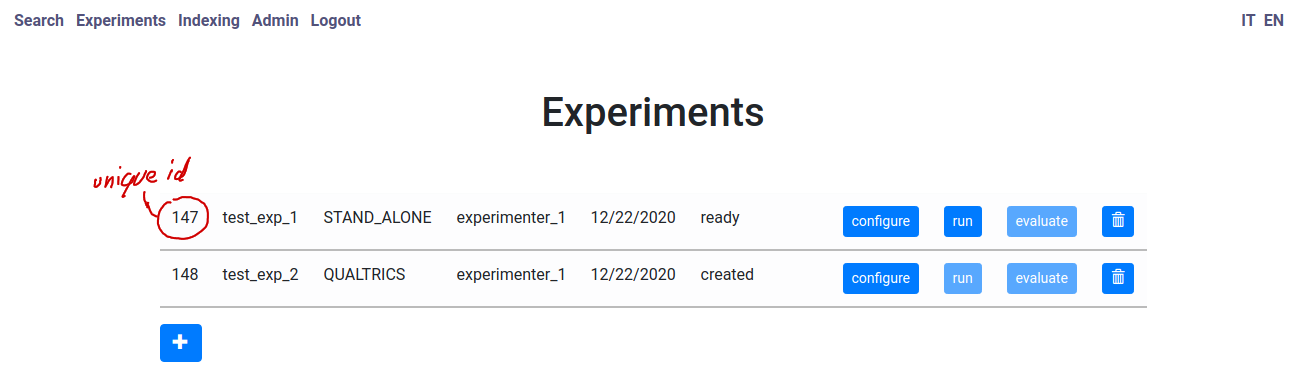
\includegraphics[width=\textwidth]{figures/experiments_1}
                 \caption{Experiments list}
                 \label{fig:experimentsUi1}
             \end{subfigure}
             \par\bigskip
             \begin{subfigure}[b]{0.8\textwidth}
                 \centering
                 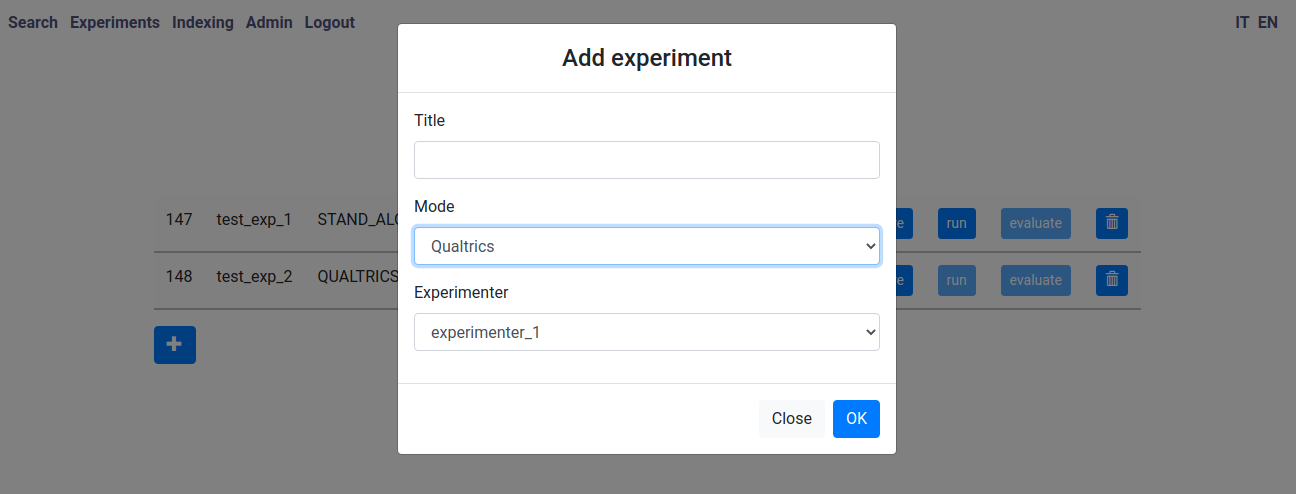
\includegraphics[width=\textwidth]{figures/experiments_2}
                 \caption{Popup for defining a new experiment}
                 \label{fig:experimentsUi2}
             \end{subfigure}
             \caption[]{Interface for defining experiments}
             \label{fig:experimentsUi}
        \end{figure}


        %%%%%%%%%%%%%%%%%%%%%%%%%%%%%%%%%%%%%%%%%%%
        \subsection{Experiment Configuration \small{(/experiments/setup/ui)}}

        The interface for experiment configuration is reachable by clicking on the \emph{configure} button in the
        experiments list UI. If the experiment's mode is \emph{stand\_alone} the configuration involves creating test groups and assigning 
        document collections and participants to them. Moreover, a document collection can be set as a predefined result list for the first query.
        Participants and groups can be defined manually or loaded from a configuration file. The same applies to \emph{Qualtrics} mode; the only difference is that 
        participants don't deed to be defined, since they are created while
        they take part in the survey.

        \subsubsection{Configuration in stand-alone mode}

        The setup UI for stand-alone experiments includes a section for uploading, inspecting, or deleting configuration files (which can be used for
        defining test groups and participants), as well as a section for editing the test groups. \textbf{Figure \ref{fig:expSetupUi1}}
        shows the page after two test groups have been added and edited; \textbf{Figure \ref{fig:expConfigFile}} shows an example of a configuration file. 
        For the configuration to be complete, i.e. its status being set to 
        \emph{complete} and the \emph{run} UI being available, there must be at least one test group defined, and each test group must 
        have some participants and at least one document collection.

        \begin{figure} [ht]
             \centering
             \hfill
             \begin{subfigure}{0.32\textwidth}
                 \centering
                 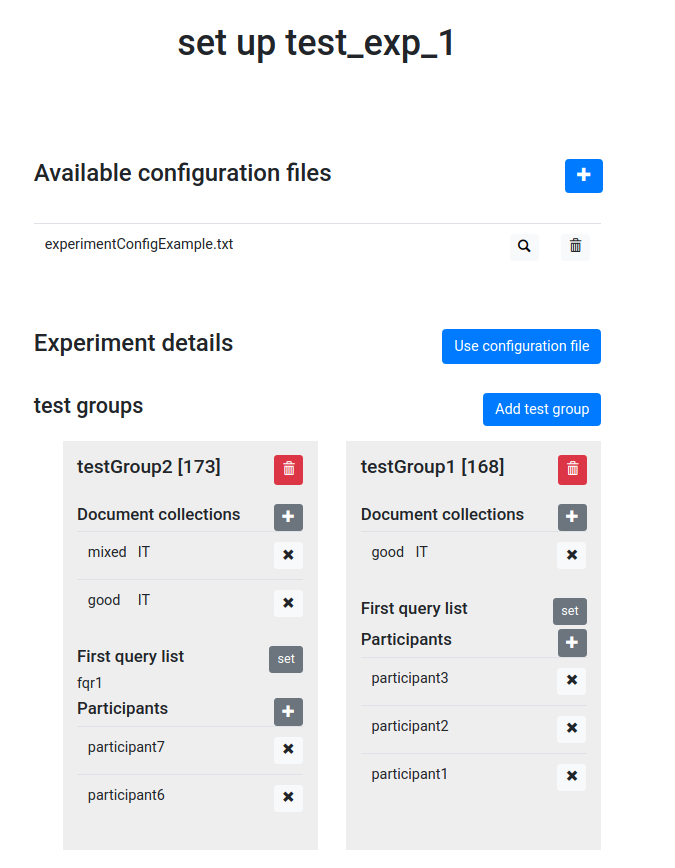
\includegraphics[width=\textwidth]{figures/expSetup1}
                 \caption{Experiment setup UI for stand-alone mode}
                 \label{fig:expSetupUi1}
             \end{subfigure}
             \hfill
             \begin{subfigure}{0.5\textwidth}
                 \centering
                 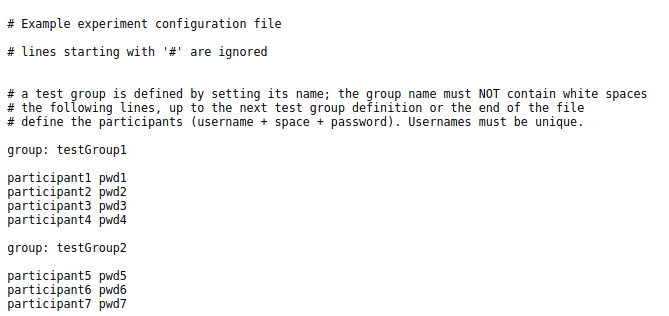
\includegraphics[width=\textwidth]{figures/expConfigFile}
                 \caption{Example of a configuration file}
                 \label{fig:expConfigFile}
             \end{subfigure}
             \hfill
             \caption[]{Experiment Configuration File}
             \label{fig:expConfigUi1}
        \end{figure}

        \newpage

        \subsubsection{Configuration in Qualtrics mode}

        In Qualtrics mode the setup options are similar, but the participants don't need to be specified, as they are defined during the survey.
        So there is no need for configuration files. For the configuration to be complete, there must be at least one test group, and each test group
        must have at least one document collection. 

        \textbf{Figure \ref{fig:expSetupUi2}} shows the configuration interface after creating and editing
        two test groups. Notice the test group's id number: this will be needed when setting up the related Qualtrics survey. 

        \begin{figure} [h]
        \centering
        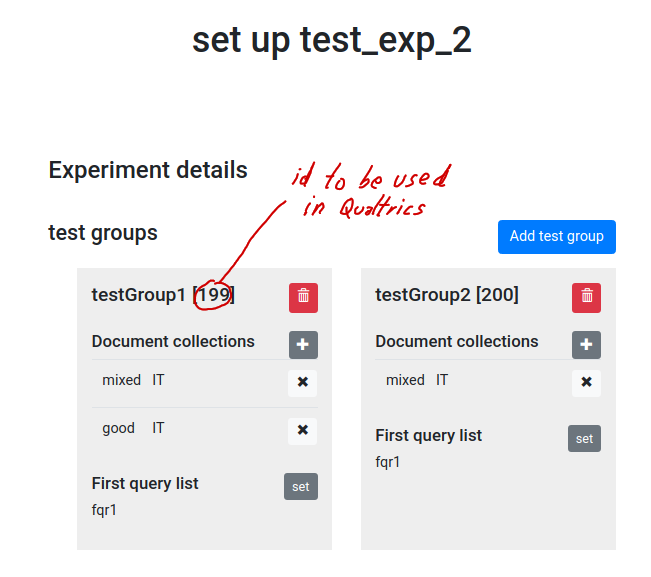
\includegraphics[width=0.5\textwidth]{figures/expSetupUi2}
        \caption[]{Experiment setup UI for Qualtrics mode}
        \label{fig:expSetupUi2}
        \end{figure}

        %%%%%%%%%%%%%%%%%%%%%%%%%%%%%%%%%%%%%%%%%%%
        \subsection{Experiment Execution \small{(/experiments/run/ui)}}

        If an experiment is configured, the related execution UI becomes available. The interface is quite simple: there is a button
        for starting, stopping, and resetting the experiment, as well as live updated information on participant's activities.
        In stand-alone mode, all participants are listed from the beginning, while in Qualtrics mode they appear as they log in.

        The purpose of the start / stop mechanism is to enable participant access and to measure the experiment's duration. As
        soon as the experiment is started, participants can lo in; when the experiment is stopped they are automatically logged out.
        In case the experiment is defined in Qualtrics mode, the participants are redirected back to the survey.
        After an experiment is started, the page can be left and returned to later.
        \textbf{Figure \ref{fig:expRunUi}} shows the interface for running an experiment.

        \begin{figure} [h]
        \centering
        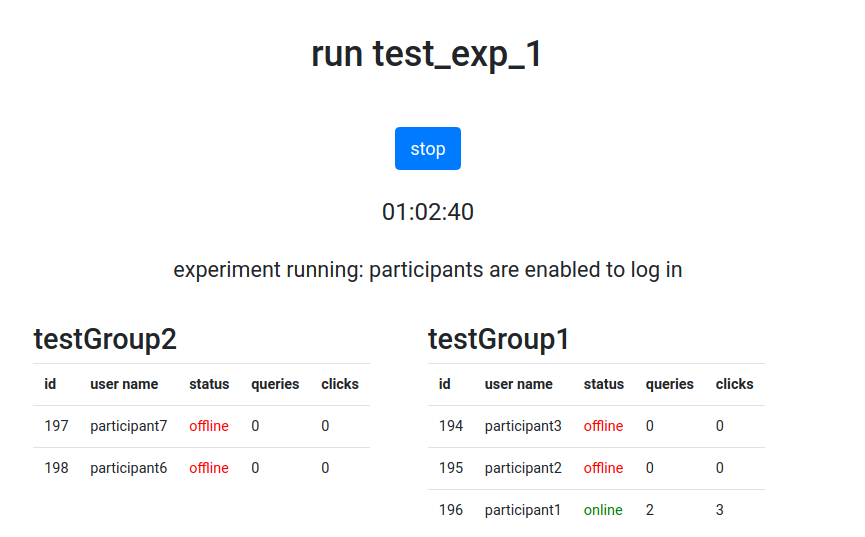
\includegraphics[width=0.5\textwidth]{figures/expRunUi}
        \caption[]{Experiments run UI}
        \label{fig:expRunUi}
        \end{figure}

        %%%%%%%%%%%%%%%%%%%%%%%%%%%%%%%%%%%%%%%%%%%
        \subsection{Setting up a linked Qualtrics survey}\label{sec:usageSurvey}

        For linking a survey to an experiment, the survey must contain
        a block whose ``next'' button redirects to HSE, a failure block to be displayed in case accidentally the experiment is not running, or
        there is some connection error,
        and some settings at the beginning of the \emph{Survey flow}. 

        \subsubsection{Survey Questions}

        The redirection is set via \emph{JavaScript} in the survey question (see
        \textbf{Figure \ref{fig:qualtricsLinkJs}}). The failure block needs no specific configuration.

        \begin{figure} [h]
             \centering
             \hfill
             \begin{subfigure}[c]{0.3\textwidth}
                 \centering
                 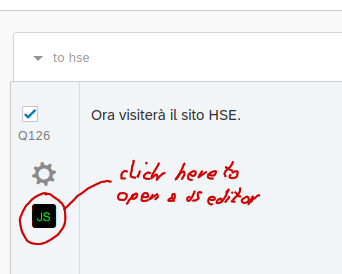
\includegraphics[width=\textwidth]{figures/qsl1}
                 \caption{Opening the JS editor}
                 \label{fig:qsl1}
             \end{subfigure}
             \hfill
             \begin{subfigure}[c]{0.35\textwidth}
                 \centering
                 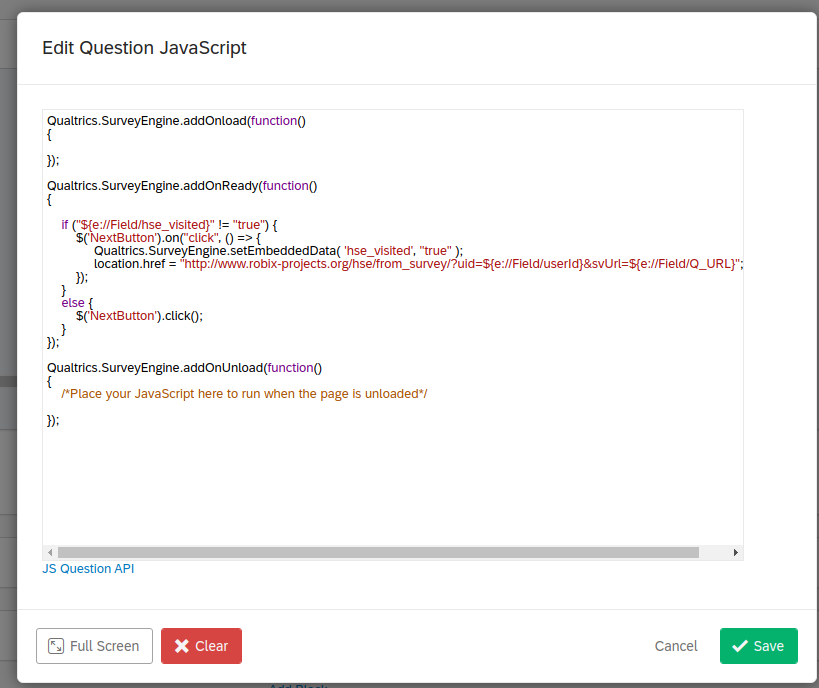
\includegraphics[width=\textwidth]{figures/qsl2}
                 \caption{Edited JS}
                 \label{fig:qsl2}
             \end{subfigure}
             \hfill
             \caption[]{Link to JS Editor}
             \label{fig:qualtricsLinkJs}
        \end{figure}

        \newpage

        In the JS editor there are three default functions: \texttt{Qualtrics.SurveyEngine.addOnload(...)}, 

        \texttt{Qualtrics.SurveyEngine.addOnReady(...)},
        and \texttt{Qualtrics.SurveyEngine.addOnUnload(...)}. The first and third functions don't need to be modified, while the
        \texttt{Qualtrics.SurveyEngine.addOnReady(...)} function needs to be edited as follows:


        \begin{verbatim}
        Qualtrics.SurveyEngine.addOnReady(function()
        {
            if ("${e://Field/hse_visited}" != "true") {

                $('NextButton').on("click", () => {
                    Qualtrics.SurveyEngine.setEmbeddedData( 'hse_visited', "true" );
                    location.href = "http://[hse server url]/from_survey/ 
                                     ?uid=${e://Field/userId}&svUrl=${e://Field/Q_URL}";				   
                });
            }
            else {

                $('NextButton').click();					  
            }					  
        });
        \end{verbatim}

        \subsubsection{Survey Flow}

        The following elements are to be added at the beginning of the survey flow, in the order they are presented here:

        \begin{enumerate}

        \item
            An \emph{Embedded Data} element for initializing some variables:

            \begin{figure} [h]
            \centering
            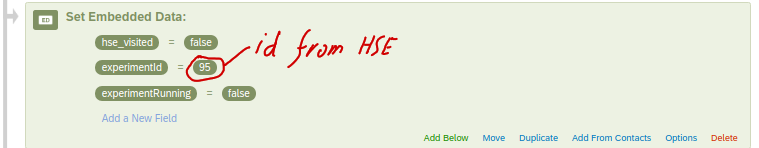
\includegraphics[width=.9\textwidth]{figures/qflow1}
            \label{fig:qflow1} 
            \caption[]{Embedded Data Element}
            \end{figure}

        \item
            A \emph{Web Service} element to do an API call for checking that the given experiment is actually running:

            \begin{figure} [h]
            \centering
            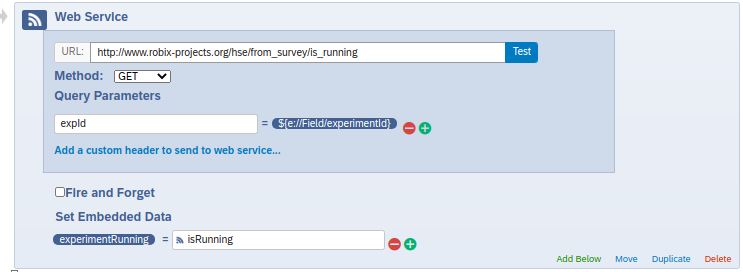
\includegraphics[width=.9\textwidth]{figures/qflow2}
            \label{fig:qflow2} 
            \caption[]{Web Service Element}
            \end{figure}

        \newpage

        \item
            A \emph{Branch} element to interrupt the survey if the experiment is not running:

            \begin{figure} [h]
            \centering
            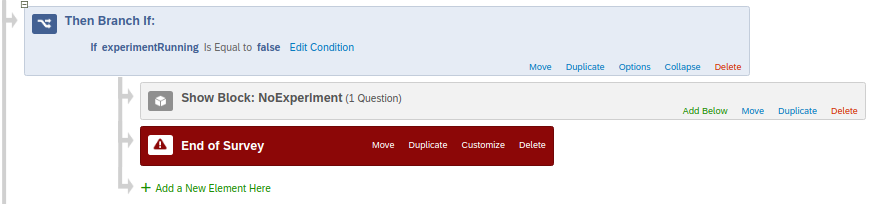
\includegraphics[width=.9\textwidth]{figures/qflow3}
            \label{fig:qflow3} 
            \caption[]{Branch Element}
            \end{figure}

        \item
            A \emph{Randomizer} element for assigning participants to test groups:

            \begin{figure} [h]
            \centering
            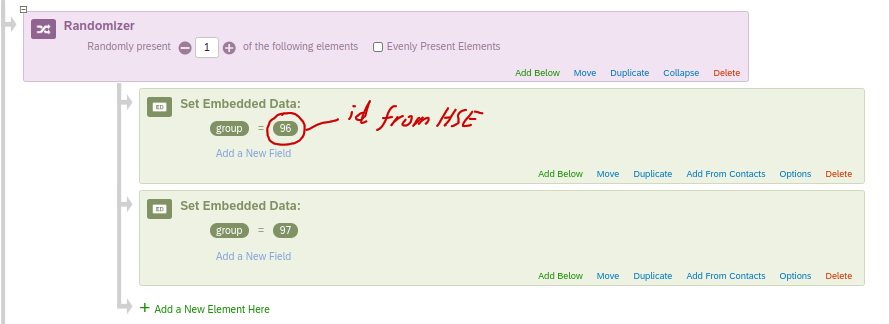
\includegraphics[width=.9\textwidth]{figures/qflow4}
            \label{fig:qflow4} 
            \caption[]{Randomizer Data element}
            \end{figure}

        \item
            A \emph{Web Service} element for initializing the participant in HSE:

            \begin{figure} [h]
            \centering
            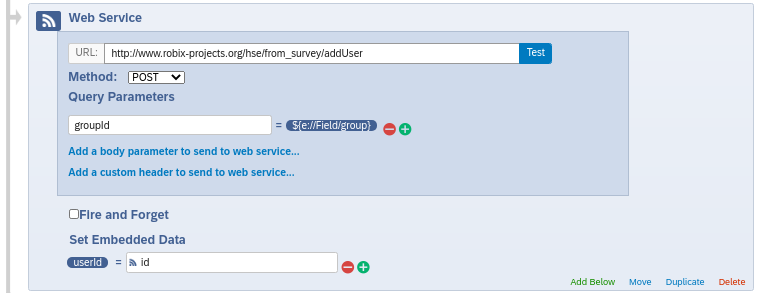
\includegraphics[width=.9\textwidth]{figures/qflow5}
            \label{fig:qflow5} 
            \caption[]{Web Service element}
            \end{figure}

        \end{enumerate}

        \vspace{.5cm}

        \textbf{Figure \ref{fig:qflow}} shows the entire edited survey flow.


        \begin{figure} [h]
        \centering
        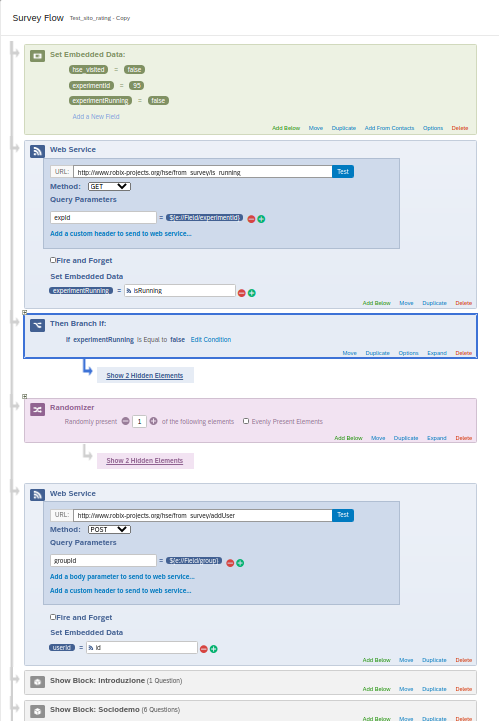
\includegraphics[width=.9\textwidth]{figures/qflow}
        \caption[]{Edited Survey Flow}
        \label{fig:qflow}
        \end{figure}

        \newpage


        %%%%%%%%%%%%%%%%%%%%%%%%%%%%%%%%%%%%%%%%%%%
        \subsection{Experiment Evaluation and Data Export \small{(/experiments/eval/ui)}}

        Once an experiment is completed, its evaluation page is accessible. The page contains several links for downloading the raw or
        partially pre-processed data, as well as a summary including per-user means and standard deviations for relevant derived data such as
        the number of documents visited, the time spent on a document, and the distribution of these measures over the different
        document collection.

        \subsubsection{Data Representation}

        The data collected during an experiment consists of a list of \emph{Usage Events}. There are three kinds of such events:
        \emph{Session Events} (login and logout), \emph{Query Events} (generated when a participant submits a search query),
        and \emph{Document Click Events} (generated when a participant clicks on a link from the results list and visits a page).
        All \emph{Usage Events} contain the following data fields:

        \begin{itemize}

        \item A unique id (generated by the database system).

        \item A timestamp of the moment when the event was generated.

        \item The user id of the participant who generated the event.

        \item The id and name of the test group the participant belongs to

        \item The event type (one of \texttt{SESSION}, \texttt{QUERY}, or \texttt{DOC\_CLICK})

        \end{itemize}

        \emph{Session Events} contain an additional field indicating whether it was a login or logout event; 
        \emph{Query Events} contain the query string submitted, the total number of retrieved results, and the proportions
        in which the document collections are represented in the results.
        \emph{Document Click Events} contain the document's URL, an id, the name and id of the collection the document belongs to,
        and its rank (position within the query results). 

        The experiment's evaluation page allows to download the entire raw data in a single \texttt{.csv} or \texttt{.json} file, 
        or the same data split into per-user histroies (in a single \texttt{.json}, or in separate \texttt{.csv} files).



        \end{appendices}


\newpage
	
%%%%% BIBLIOGRAPHY %%%%%
\bibliographystyle{abbrv}
\bibliography{references}

\end{document}





















